\documentclass{article}

\linespread{1.5}
\usepackage[utf8]{inputenc}
\usepackage[left=1.35in,right=1.35in,bottom=0.85in]{geometry}
\setlength\parindent{0pt}
\setlength{\parskip}{1em}
\setcounter{secnumdepth}{0}
\usepackage{outlines}
\usepackage{graphicx}
\graphicspath{ {imgs} }
\usepackage[hyphens]{url}
\usepackage{hyperref}
\usepackage{color,soul}
\usepackage[normalem]{ulem}
\usepackage{tabularx}
\usepackage{pgfgantt}
\usepackage[toc]{appendix}
\usepackage{comment}

\usepackage[
backend=biber,
style=apa,
citestyle=authoryear,
sorting=nyt,
]{biblatex}
\addbibresource{refs.bib}

\newcommand{\alignedmarginpar}[1]{%
        \marginpar{\raggedright\small #1}
    }
    
\newcommand{\bisection}[1]{\textbf{\textit{#1}}}

\DeclareCiteCommand{\citeyear}
    {}
    {\bibhyperref{\printdate}}
    {\multicitedelim}
    {}

\title{Research Proposal - Perceived accessibility of urban blue space in Copenhagen}
\author{Carla Hyenne}
\date{}

\begin{document}

\maketitle

\tableofcontents 

%%%%%%%%%%%%%%%%%%%%%%%%%%%%%%%%%%%%%%%%%%%
%				ABSTRACT (500 WORDS)
%%%%%%%%%%%%%%%%%%%%%%%%%%%%%%%%%%%%%%%%%%%
\pagebreak
\section{Abstract}

The benefits of urban nature on people’s health, for fostering community, and for climate change adaptation are widely acknowledged. Within the discourse of environmental justice (EJ), these benefits have been used to demonstrate that equitable access to healthy, unpolluted environments is a human right, with scholars like Anguelovski and Agyeman arguing that marginalised and vulnerable populations are disproportionately affected by lack of access to such spaces. 

Despite extensive studies on the accessibility of urban green spaces (UGS), urban blue spaces (UBS) have not been given the same attention. Moreover, research on UGS accessibility has focused on geographical accessibility, such as proximity to home, and has seldom considered subjective experiences as influencing access. However, accessibility is a multidimensional and complex concept which cannot be reduced to spatial distribution. As Wang, Brown and Liu put forward, perceived accessibility that addresses subjectivities, socio-personal characteristics, and the quality and diversity of the space, must also be considered.

My research addresses the issue of perceived accessibility to UBS by looking at the extent to which subjective experiences and perceptions shape how (un)fairly accessible high-quality, public UBS interventions are, and what this means for the environmentally just city.
I will pay special attention to socio-economic and personal characteristics such as age, gender, income, ethnicity, cultural practices, and general preferences for infrastructure and aesthetics.

Specifically, I will be looking at three blue spaces in Copenhagen located in neighbourhoods with varying socio-economic and demographic profiles. A combination of observations of human activity and site quality, and surveys with users, will allow me to study a variety of perspectives on UBS. I will discuss the extent to which the city of Copenhagen offers equitable opportunities for people with different backgrounds and preferences to enjoy UBS, and juxtapose this against the ideal of the environmentally just city. 
Given the availability of UBS in Copenhagen and the importance the city is giving to harbour baths and urban beaches, it will be particularly useful to evaluate whether Copenhagen’s UBS caters to everyone’s needs.

I argue that perceived accessibility is an important dimension of EJ, because public UBS are places of community, attachment, and well-being. Ignoring subjective experiences that differ from the mainstream can contribute to social inequalities, discrimination, and displacement.

In conclusion, my research will closely examine how perceptions shape accessibility to UBS. It will serve to understand what perceptions and experiences those who control access (city planners) must take into account if UBS are to be usable by everyone.

%%%%%%%%%%%%%%%%%%%%%%%%%%%%%%%%%%%%%%%%%%%%
%								LITERATURE REVIEW (2-3 PAGES)
%%%%%%%%%%%%%%%%%%%%%%%%%%%%%%%%%%%%%%%%%%%%
\pagebreak
\section{Literature review}

This section reviews the academic literature on urban blue spaces (UBS), and incorporates literature from wider fields like urban ecology. It also introduces concepts that are central for understanding the use of UBS, namely ecosystem services\sout{, environmental justice} and social barriers. Although a lot of the literature mentioned is focused on green spaces, the similarities between green and blue spaces with regards to social and environmental effects give grounds for judiciously extending the research to include blue spaces. Moreover, many blue spaces have some green space, and vice versa.

%%%%%%%%%%%%%%%%%%%%
\subsection{The benefits of urban blue space}
%%%%%%%%%%%%%%%%%%%%

%%% Ecosystem system services as a way to understand the value that people, and cities as a whole, can derive from urban nature
% UBS are often highlighted as providing significant ecosystem services, including cultural and regulating ecosystem services.
In an urban context, UBS has undeniable positive effects on people and the environment, which Gascon et al. (\citeyear{gascon2017outdoor}) summarise as ``stress reduction, increased physical activity, promotion of positive social contacts, increased place attachment and the reduction of extreme temperatures''. These benefits can be understood under the broad categories of health and ecosystem services. Within ecosystem services, we distinguish two realms, namely cultural and regulating.

%%% Health benefits of UBS
Firstly, UBS provide physical and mental health benefits - being exposed to water makes people feel better and be more active. There is an extensive repertoire of quantitative studies demonstrating these effects on people's health and well-being (\cite{gascon2017outdoor}, \cite{britton2020blue}), and qualitative studies also show that exposure to UBS improves mental health, regardless of how people interact with it (\cite{garrett2019urban}, \cite{van2021urban}).

%%% Cultural ES
Secondly, cultural ecosystem services refer to the intangible benefits that people derive from their relationship to nature. These benefits include recreation, cultural and spiritual practices, opportunities for education, or community forming and belonging \parencite{phillips2021use}. A recent example of people discovering the cultural value of urban blue and green spaces is the COVID-19 pandemic. During the strict lockdown measures implemented by governments worldwide, people (re)discovered the value of parks, forests, rivers and lakes as places to escape from home and interact safely with others in an open space \parencite{kohsaka2021urban}. 

\hl{TODO READ Plieninger DisentanglingEcosystemServices}

%%% Regulating ES for climate extremes
Lastly, regulating ecosystem services refer to the power that nature has to mitigate extreme events, particularly in relation to climate change. When blue and green infrastructure work in tandem, they can alleviate heat stress by acting as cooling islands (\cite{gunawardena2017utilising}, \cite{lin2020water}) or provide protection from heavy rainfall and flooding through the design of natural stormwater management systems like flood plains (\cite{o2020sustainable}, \cite{ghofrani2017comprehensive}). Moreoever, water is necessary for  any green infrastructure to sustain itself and provide well-known benefits like reducing air pollution \parencite{pugh2012effectiveness}. Thus, when planned in accordance with local environmental features, blue-green infrastructure can increase the climate resiliency of cities \parencite{o2021international}.

%%% Thesis --> benefits of UBS for biodiversity. Ref \parencite{kimic2021assessment} on biodiversity (1.2.2)

Given the potential benefits of UBS on people and the environment, providing public UBSs that meet the needs of residents contributes to creating socially and environmentally resilient cities.
 
%%%%%%%%%%%%%%%%%%%%
\subsection{The renewal of urban blue space}
%%%%%%%%%%%%%%%%%%%%

Most large cities are located near water, either inland like rivers, lakes or harbours, or on the coast. With urbanisation, these waters became polluted or transformed by industries \parencite{kampa_langaas_anzaldua_2016} and UBS became unattractive and unsafe to swim in.
In the 20th century, post-industrial European cities started considering UBSs as strategic opportunities to revitalise the city \parencite{del2021dismantling}. Over the last few decades, the importance of water in the city has entered public consciousness due in part to climate concerns, and most recently with the COVID-19 pandemic.
Through local and international political pressure and public demand, governments have invested significant resources in revitalising UBS into attractive places for people to use.

\subsubsection{Positive effects of urban blue space renewal}

UBS renewal projects can provide specific social benefits in addition to the aforementioned cultural ecosystem services, namely community building.
%%% Ways in which UBS renewal is positive: building community; cleaning up polluted spaces;
UBSs give people the opportunity to connect with each other, and renewal projects are an opportunity to create form community by engaging residents in the design and implementation process. In a deprived area of Plymouth, in the UK, a small-scale UBS intervention revealed that residents who participated in the project reported a greater sense of well-being and life satisfaction due to feelings of community belonging and an increased sense of safety in their neighbourhood \parencite{van2021urban}.

%%% TODO something more about ubs renewal benefits??

%%% Bring in EJ? as a principle which illustrates the need to provide safe, clean, unpolluted environments for all

%%%%%%%%%%%%%%%%%%%%
\subsubsection{Social consequences of urban blue space renewal}
%%%%%%%%%%%%%%%%%%%%
% thesis --> add "and the environment" and clarify how improvements to UBS can harm environment

Despite the undeniable benefits of water in the city, upgrading UBSs into clean and attractive public spaces can have undesirable social consequences.
Two mechanisms of action are exclusionary planning and the effect on green (or blue) gentrification.
% \sout{These reinforce socio-spatial inequalities by discriminating against people on the basis of socio-economic and cultural differences, or by way of racist and sexist practices.}

%%% Exclusionary planning can disrupt local communities
First, in contrast to the social bonds that can be fostered when residents are involved in renewal projects, UBS interventions can disrupt connections between people and with nature.
This is exacerbated by the tendency to view polluted or degraded UBS as having less value than clean and attractive spaces \hl{parencite REF}. 
However, Toomey et al. (\citeyear{toomey2021place}) demonstrate in their research on Coney Island Creek in New York City that people can attach meaning to degraded UBS. Despite the water being heavily polluted, the Creek supports a range of activities and social connections, and there were concerns from local experts that future urban renewal may disrupt these practices. One way to overcome this is for planners to consult the local community during the design and implementation of any UBS intervention.

However, marginalised or stigmatised communities may find it hard to communicate their experience when consulted by planners, because they lack a common language to articulate their reality. And vice-versa: wealthy, white, males may not be capable of understanding the experience of `others' \parencite{anguelovski2020expanding}. To this end, Toomey et al. (idib.) propose using language like ``place-disruption'' and ``place-protection'' to promote mutual understanding and avoid privileging the values of mainstream groups over those of marginalised communities.

%%% Effects of UBS renewal on the housing market/`green' gentrification
Second, local governments are using UBS to brand their cities as `green' and liveable.
\hl{need to explain how this relates to greening as winwin} Two examples are Madrid promoting the Madrid Río project on the official tourism website \parencite{madridrio}, or Oslo advertising its new urban waterfront promenade along which you can admire the city's starchitecture \parencite{visitoslo}.

Cities are also using greening, the process of upgrading urban settings into environmentally more sustainable spaces,  as a win-win strategy where ``no one is left behind by the trickle-down of benefits from green infrastructure'' \parencite{anguelovski2021green}. However, there is a mismatch between cities trying to attract new creative classes through UBS renewal, and with addressing UBS as a common good and prioritising the concerns of existing residents (\cite{wessells2014urban}, \cite{anguelovski2020expanding}).

These strategies can perpetuate inequalities by privileging the values of white, environmentally privileged upper classes who can afford to live near nature \parencite{REF} \hl{REF}. This phenomenon is referred to as green gentrification, where greening can contribute to the exclusion and displacement of residents, who are priced out to a neighbourhood with less attractive nature.

\begin{comment}
%%%%%%%%%%%%%%%%%%%%
\subsection{The environmental justice principle} % making sense of conflicting benefits and consequences of UBS renewal
%%%%%%%%%%%%%%%%%%%%
\alignedmarginpar{But is EJ still useful here?}

To articulate the phenomenon whereby UBSs provide social and environmental benefits, but at the same time discriminate against vulnerable populations, scholars have used the concept of environmental justice (EJ).
EJ has evolved into the principle that everyone should have equal opportunities to access clean, healthy, unpolluted spaces, and in turn, share environmental burdens. As Agyeman et al. explain (\citeyear{agyeman2016trends}), it started as a social movement in the US in the 1980s at a time when it became obvious that ethnic minority and low-income populations were disproportionately exposed to polluted and degraded land.

Since then, EJ has concretised into an academic discourse that looks at a range of UBS factors such as the location of UBS in the city, discrimination in public participation and decision making with regards to UBS renewal, and individual and community perceptions and preferences which may influence how people interact, or not, with the space.
% thesis -->  argue that sustainability not being only enviro but also eco and social, and \parencite{agyeman2016trends}

% todo --> expand on importance of blue space being understudied
The applications of EJ on UBS are limited in comparison to urban green space. One study that stands out is Raymond et al.'s (\citeyear{raymond2016integrating}) research on the diversity of people, activities and perceived unpleasant experiences in Helsinki's blue spaces. The wide range of opinions they find show the importance of considering a multitude of perceptions when planning UBS, because people of different age, income, gender, ethnicity, etc. have varying preferences.

%%% EJ takes place in public spaces, but public spaces aren't always possible to use by everyone
It follows that environmental (in)justices take place in public space, where people can freely use the space. However, not having an entrance fee to UBS does not mean that everyone feels like they have the possibility to use the space. There are a multitude of barriers, either physical or perceived, that can inhibit the use of public space.
\end{comment}

%%%%%%%%%%%%%%%%%%%%
\subsection{Making use of urban blue space}
%%%%%%%%%%%%%%%%%%%%

%%% How people can get access to the benefits of CES
Using UBS is the one way to reap the health and social benefits aforementioned. And for people to engage with UBS, they must be available. However, their availability doesn't guarantee that unique individual needs will be fulfilled \parencite{phillips2021use}. There are a variety of factors that go into deciding whether or not a space is attractive. For example, in their research, Phillips et al. (ibid.) analyse people's motivations and preferences for using particular green spaces in Brussels. They find that there are two distinct groups of people: those who use parks to be close to nature, and those who go to parks to be surrounded by people. Thus, the presence and reachability of UBS aren't sufficient to determine use, and renewal projects need to consider socio-personal nuances.

For analysing the use of green space, Biernacka and Kronenberg (\citeyear{biernacka2018classification}) propose looking at their availability, accessibility and attractiveness as shown in figure ~\ref{fig:diagram_ubs_use}.
Availability refers to the physical presence of green space, whereas accessibility refers to the physical and perceived reachability of the space - whether it can be reached in reasonable time, or if it is seen as open and public (not private). 
They argue that the first two, availability and accessibility, must be fulfilled before people can evaluate attractiveness and consider using the space. 
It follows that an abundance of UBS does not necessarily mean that demand is met, if individual needs are not satisfied.

\begin{figure}[h]
	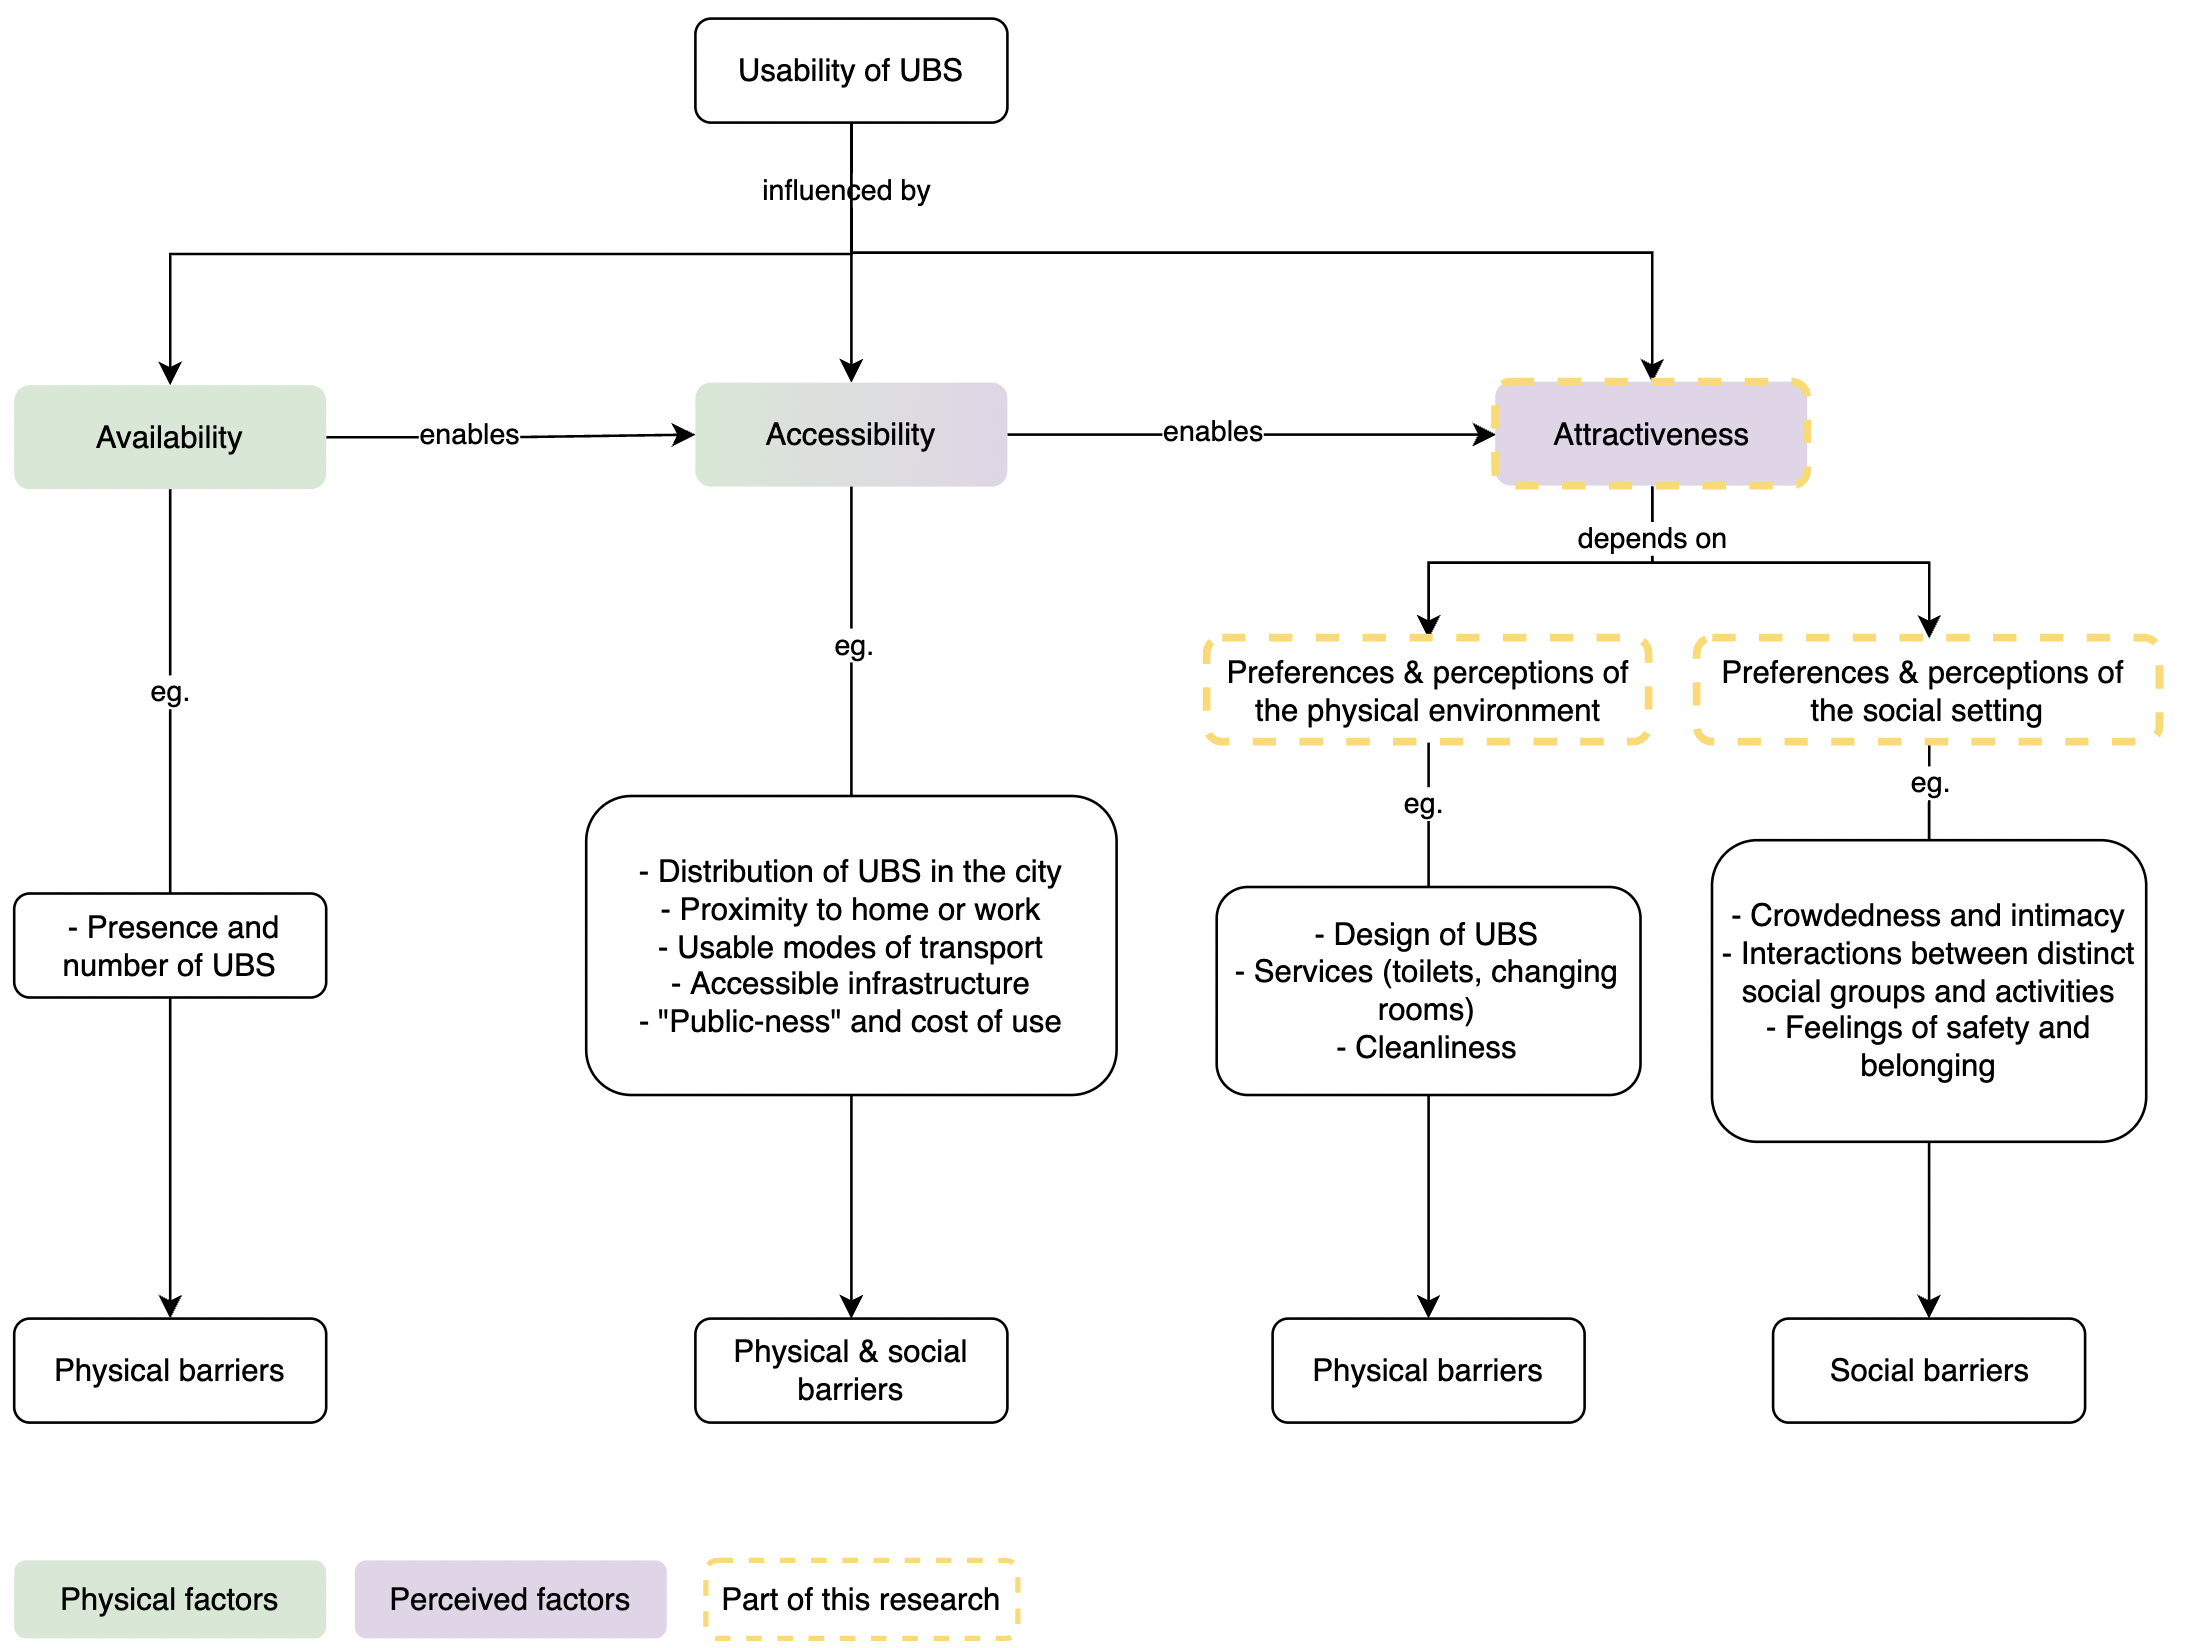
\includegraphics[width=\textwidth]{diagram_ubs_use.png}
	\caption{\textit{A diagram summarising the three factors influencing usability of UBS - availability, accessibility and attractiveness - along with examples of barriers that influence the fulfillment of these factors.}}
	  \label{fig:diagram_ubs_use}
\end{figure}

%%% Influence of demographic data
Specifically influential in determining the use of UBS are socio-economic factors like age, sex, income, and education levels \parencite{REF}. In neighbourhoods with lower socio-economic status the use of green space is often lower than in more affluent neighbourhoods, despite similar opportunities to access green spaces \parencite{REF}. This mismatch between provision and use can be explained by perceived accessibility and social barriers preventing people from finding the space attractive (\cite{wang2015comparison}, \cite{noel2021social}).

\subsubsection{Barriers to using UBS}

Barriers are understood as anything that prevents people from using, or feeling like they can use, UBS.
These barriers can be physical, such as the existence of UBS in the city, their distribution, their accessibility by different modes of transit, or their distance from home (\cite{REF}, \cite{REF}). Barriers can also be non-physical, such as perceptions and preferences in the built environment and services, in the types of activities and people using the space, or feelings of safety or belonging \parencite{REF}.

To date, studies that evaluate the degree to which people can make use of urban nature have focused not only on green spaces, but also on measuring geographical factors like availability and physical accessibility.
However, the reasons for using green spaces or UBS are complex and multidimensional, and cannot be reduced to a purely physical aspect \parencite{wang2015physical}. There are a multitude of socio-personal factors also at play, shaped by perceptions and subjective experiences.

To this end, Wang et al. (\citeyear{wang2015physical}) suggest focusing on factors that influence perceptions of green space, ie. ``the quality, diversity, and size of the green spaces or socio-personal characteristics including age, income, safety, and cultural concerns''. In their research on public parks in Brussels, Noel et al. (\citeyear{noel2021social}) focus on social barriers and show that they influence the ways and the extent to which people use the parks.
\hl{explain more social barriers?}
% like feelings of belonging and safety, preferences in social settings, XX, or XX. They show that social barriers influenced the ways in which people made use of green spaces


\subsection{Research intention}

While there is considerable research on the physical barriers, and to some extent social barriers to green space, studies focusing on UBS are limited.
However, UBS are particularly interesting because natural water bodies like rivers or lakes are relatively immobile and cannot be planned in the same way as public parks.
Thus, when it comes to designing strategies to create equal opportunities to use UBS, perceived factors become more relevant than physical factors. 
This makes it worthwhile to explore the subjective experiences of UBS users, in order to understand what social barriers exist in the context of blue space, \sout{and how to create effective policies for increasing the use of UBS for everyone.}

%%%%%%%%%%%%%%%%%%%%%%%%%%%%%%%%%%%%%%%%%%%%%%
%								PROBLEM STATEMENT AND RQ (1 PAGE)
%%%%%%%%%%%%%%%%%%%%%%%%%%%%%%%%%%%%%%%%%%%%%%

\section{Problem Statement}

% Ideal
The principle of environmental justice entails equitable access to clean, unpolluted environments, such as high-quality public UBS. This is important because exposure to water bodies improves people's health and well-being, and being at the waterfront can build relationships within a neighbourhood or community.
% Real
In reality, a multitude of barriers exist which may prevent individuals or communities from visiting UBS even if they live nearby. The barriers include physical characteristics like preferences for the quality, size, or infrastructure of the site; and non-physical characteristics like socio-economic and personal factors including income, age, gender, ethnicity or cultural concerns.
% Consequences
Understanding this phenomenon is important because public UBS are places of community, identity, attachment, and well-being. Ignoring subjective experiences that differ from the mainstream can contribute to social inequalities, discrimination, and displacement.

% Research question
Given the above, my research aims to answer the following question: \textbf{to what extent do subjective experiences and perceptions shape how (un)fairly usable high quality, public blue space interventions are, and what does this mean for the environmentally just city?}

I define high quality UBS as \hl{TODO}

%%%%%%%%%%%%%%%%%%%%%%%%%%%%%%%%%%%%%%%%%%%%%%
%							RESEARCH DESIGN (4-6 PAGES)
%%%%%%%%%%%%%%%%%%%%%%%%%%%%%%%%%%%%%%%%%%%%%%
\section{Methodology}

\sout{My research will be explanatory because I aim to explain whether or not there are equal opportunities for people to access UBS. I will take an inductive approach, whereby my theory will emerge from the data I will collect on people’s uses and perceptions of UBS, and on the quality and diversity of the sites. The theories framing the research are environmental justice - everyone should have equal access clean, unpolluted, healthy environments - and perceived accessibility - the subjective, socio-personal, preferential characteristics that shape access}

%%%%%%%%%%%%%%%%%%%%
\subsection{Case study}
%%%%%%%%%%%%%%%%%%%%

The research will compare perceived barriers to UBS in three different UBS in the city of Copenhagen.

\subsubsection{The context of Copenhagen}

To assess the opportunities residents have to use UBS in everyday life, the sites should be located in a single city. Copenhagen makes for an interesting case for the following four reasons. First, Copenhagen is located on the Kattegat strait, has a high availability of UBS with 92 km of coastline, and water features prominently in the urban landscape \parencite{comertler2017greens}. Second, the city trying to position itself as a world leader in sustainability and is doing so by making its shoreline attractive. Since 2002, there have been over ten blue space rehabilitation projects in the form of harbour baths and urban beaches, which are now open to the public and free to use \parencite{visitcopenhagen_baths}. Third, Copenhagen is experiencing an increase in poverty and ethnic segregation \parencite{moller2015socioeconomic}, as well as a growing racist discourse in the media and politics. For example, through the classification of some neighbourhoods as ‘ghettos’ \parencite{simonsen2008practice}. This evolving socio-economic landscape and its surrounding discourse make it important to understand who feels like they can access UBS, and who might not. Finally, Copenhagen’s reputation as one of ``the most liveable cities'' \parencite{visitdenmark_2021}, due in part to the swimming spots in the harbour, begs the question - for whom is the city liveable, if not all can use the UBS?

\hl{TODO: map distance of UBS to place of residence/400m from building blocks}

\subsubsection{Potential cases}

\hl{Define UBS, high-quality}

Specific units of analysis must be defined. Every UBS and neighbourhood will have a different set of social, economic, political, cultural or environmental conditions which influence who uses the space, why, and how they feel. In order to uncover these conditions, the units of analysis should be scoped to specific locations on the waterfront, and match three criteria. 

First, the UBS should allow people to carry out a multitude of activities like sitting, swimming, eating, playing sports, sunbathing, etc. to make sure people can carry out the activity they want in the space.
Second, the sites should have been rehabilitated by the city, be public and free to use.
Third, because perceived accessibility is rooted in socio-economic, cultural and personal factors, the UBS should be located in neighbourhoods distinct socio-economic status. Social economic status (SES) has been recognised as influencing perceived access to green space, with scholars like Wang, Brown and Liu showing that people in neighbourhoods with lower SES have lower perceived accessibility to parks (\citeyear{wang2015physical}). \hl{Add Cronin-de-Chavez research}

The maps in figure ~\ref{fig:map_income} represent income and education statistics of districts in Copenhagen, retrieved from Denmark's statistic bank \parencite{copenhagenStatbank}. These statistics, along with the list of harbour baths and beaches on the VisitCopenhagen website \parencite{visitcopenhagen_baths}, served to shortlist five UBS: the Sandkaj harbour bath, the Svanemøle beach, the Sluseholmen harbour bath, the Amager beach and the Kastrup sea bath (see Figure ~\ref{fig:ubs}). I will likely not be able to analyse five spaces, but a more detailed neighbourhood analysis and a visit to the spaces is required to make a final decision. 

I also considered inland UBS such as lakes or rivers, which would be interesting to compare with the high-profile harbours and beaches. However I could not identify any that supported many activity (ie., it was not possible to swim, play sports, sit, etc.). Visiting these spaces in person might change my interpretation.

\begin{figure}[h]
	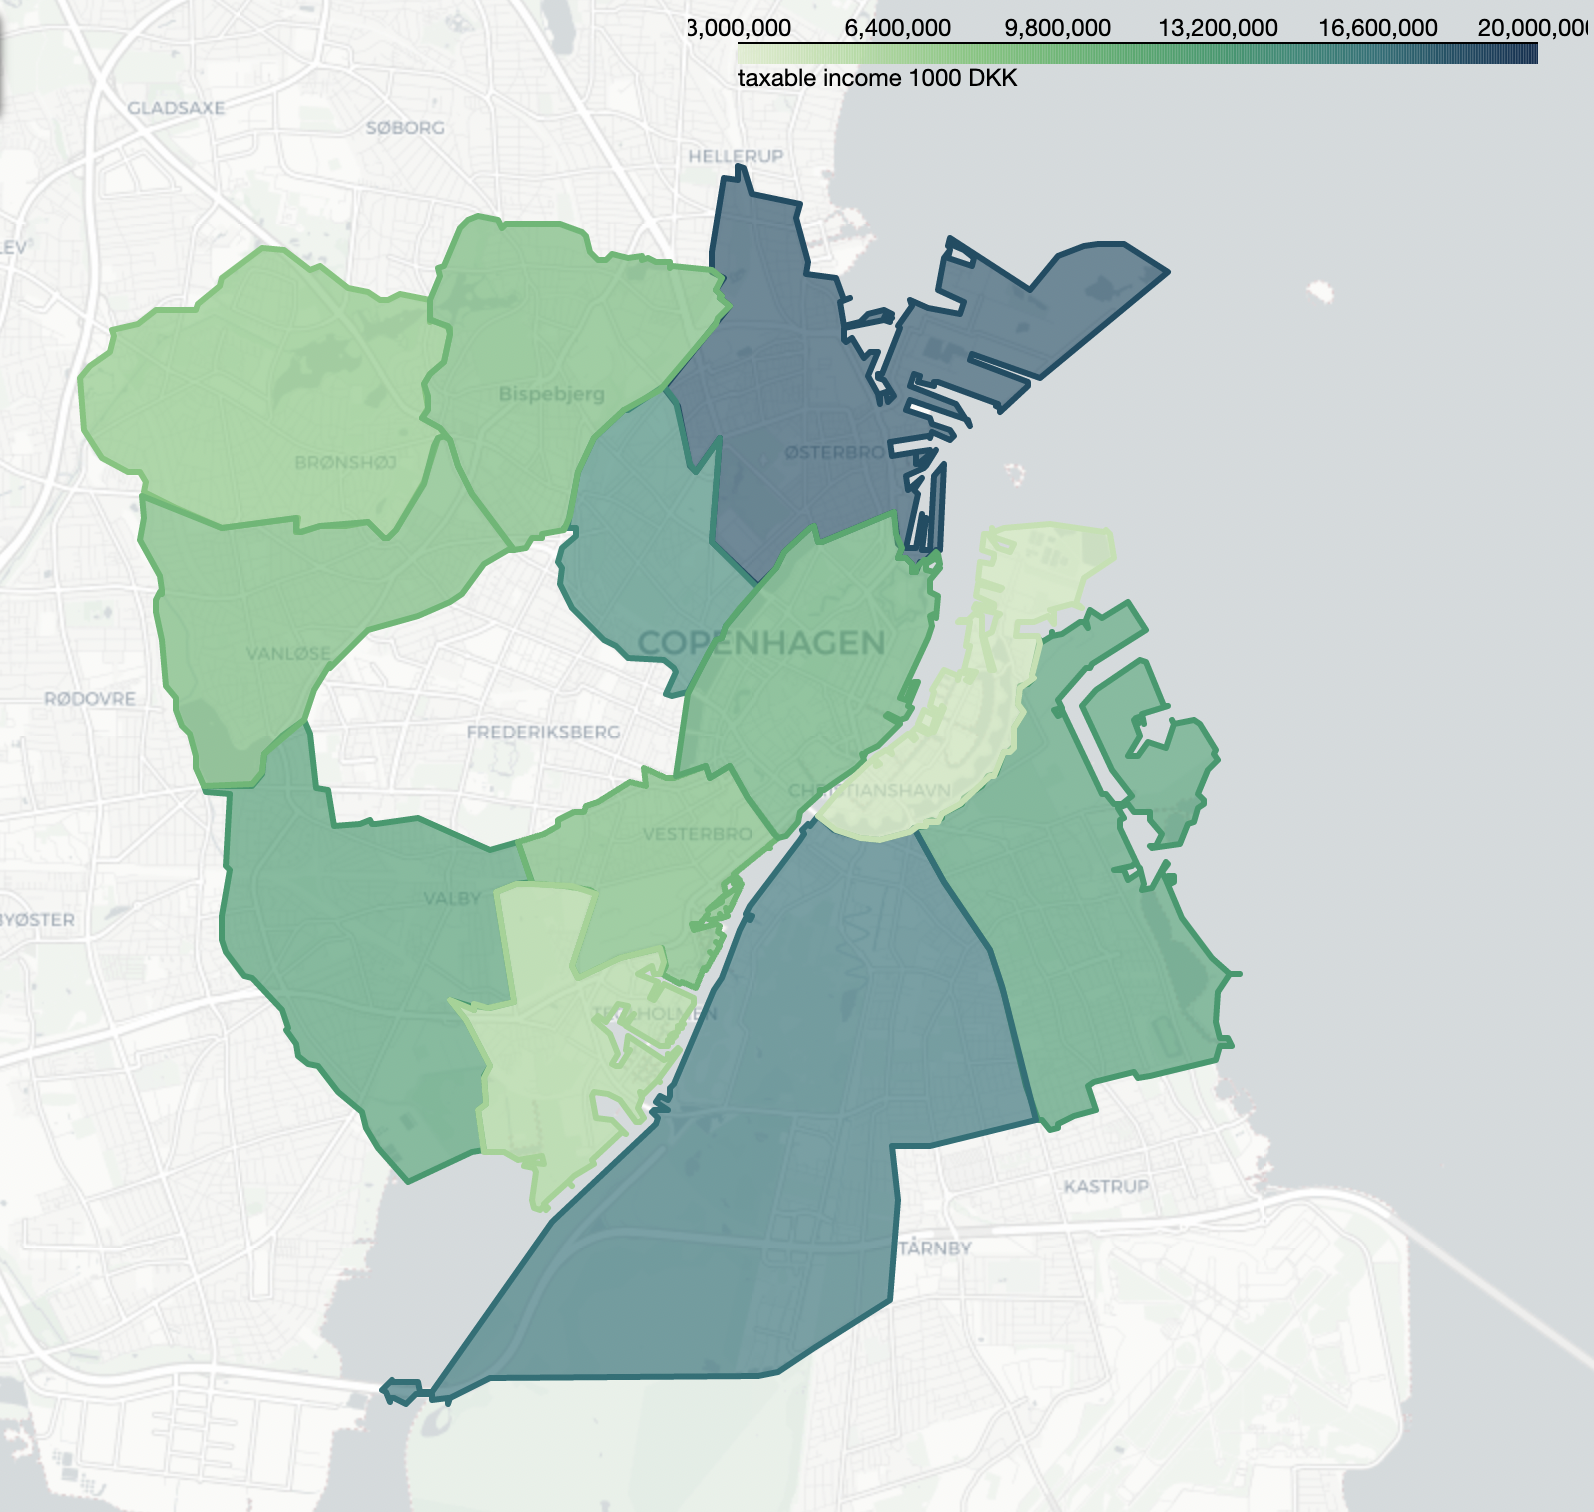
\includegraphics[width=0.5\textwidth]{copenhagen_income_taxable.png}
	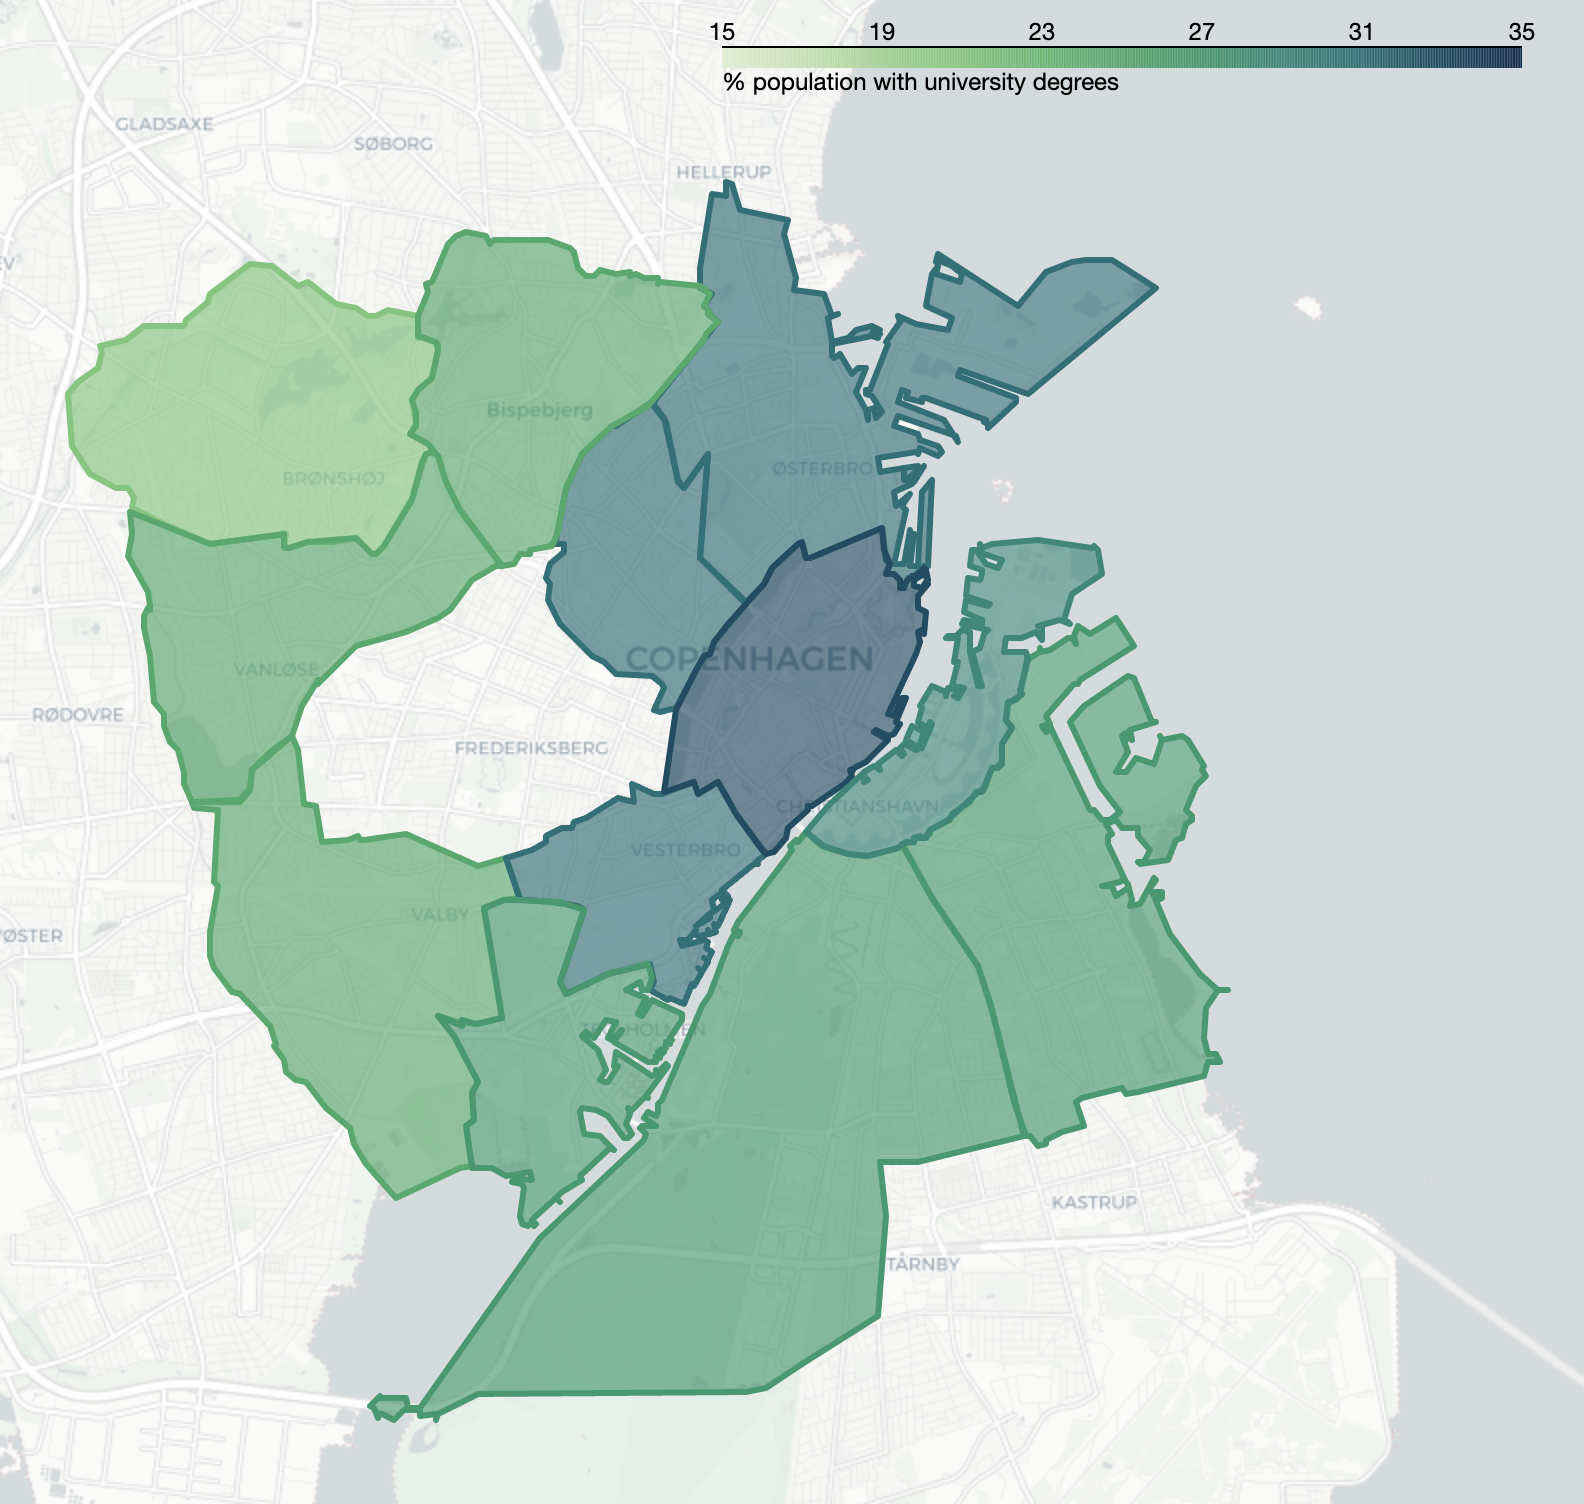
\includegraphics[width=0.5\textwidth]{copenhagen_edu.png}
	\caption{\textit{Left: taxable income (in 1000 DKK) the districts of Copenhagen for the year 2020. Right: percentage of residents with a university degree (Bachelor, Master or PhD) in the districts of Copenhagen for the year 2020.}}
	  \label{fig:map_income}
\end{figure}

\begin{figure}[h]
	\centering
	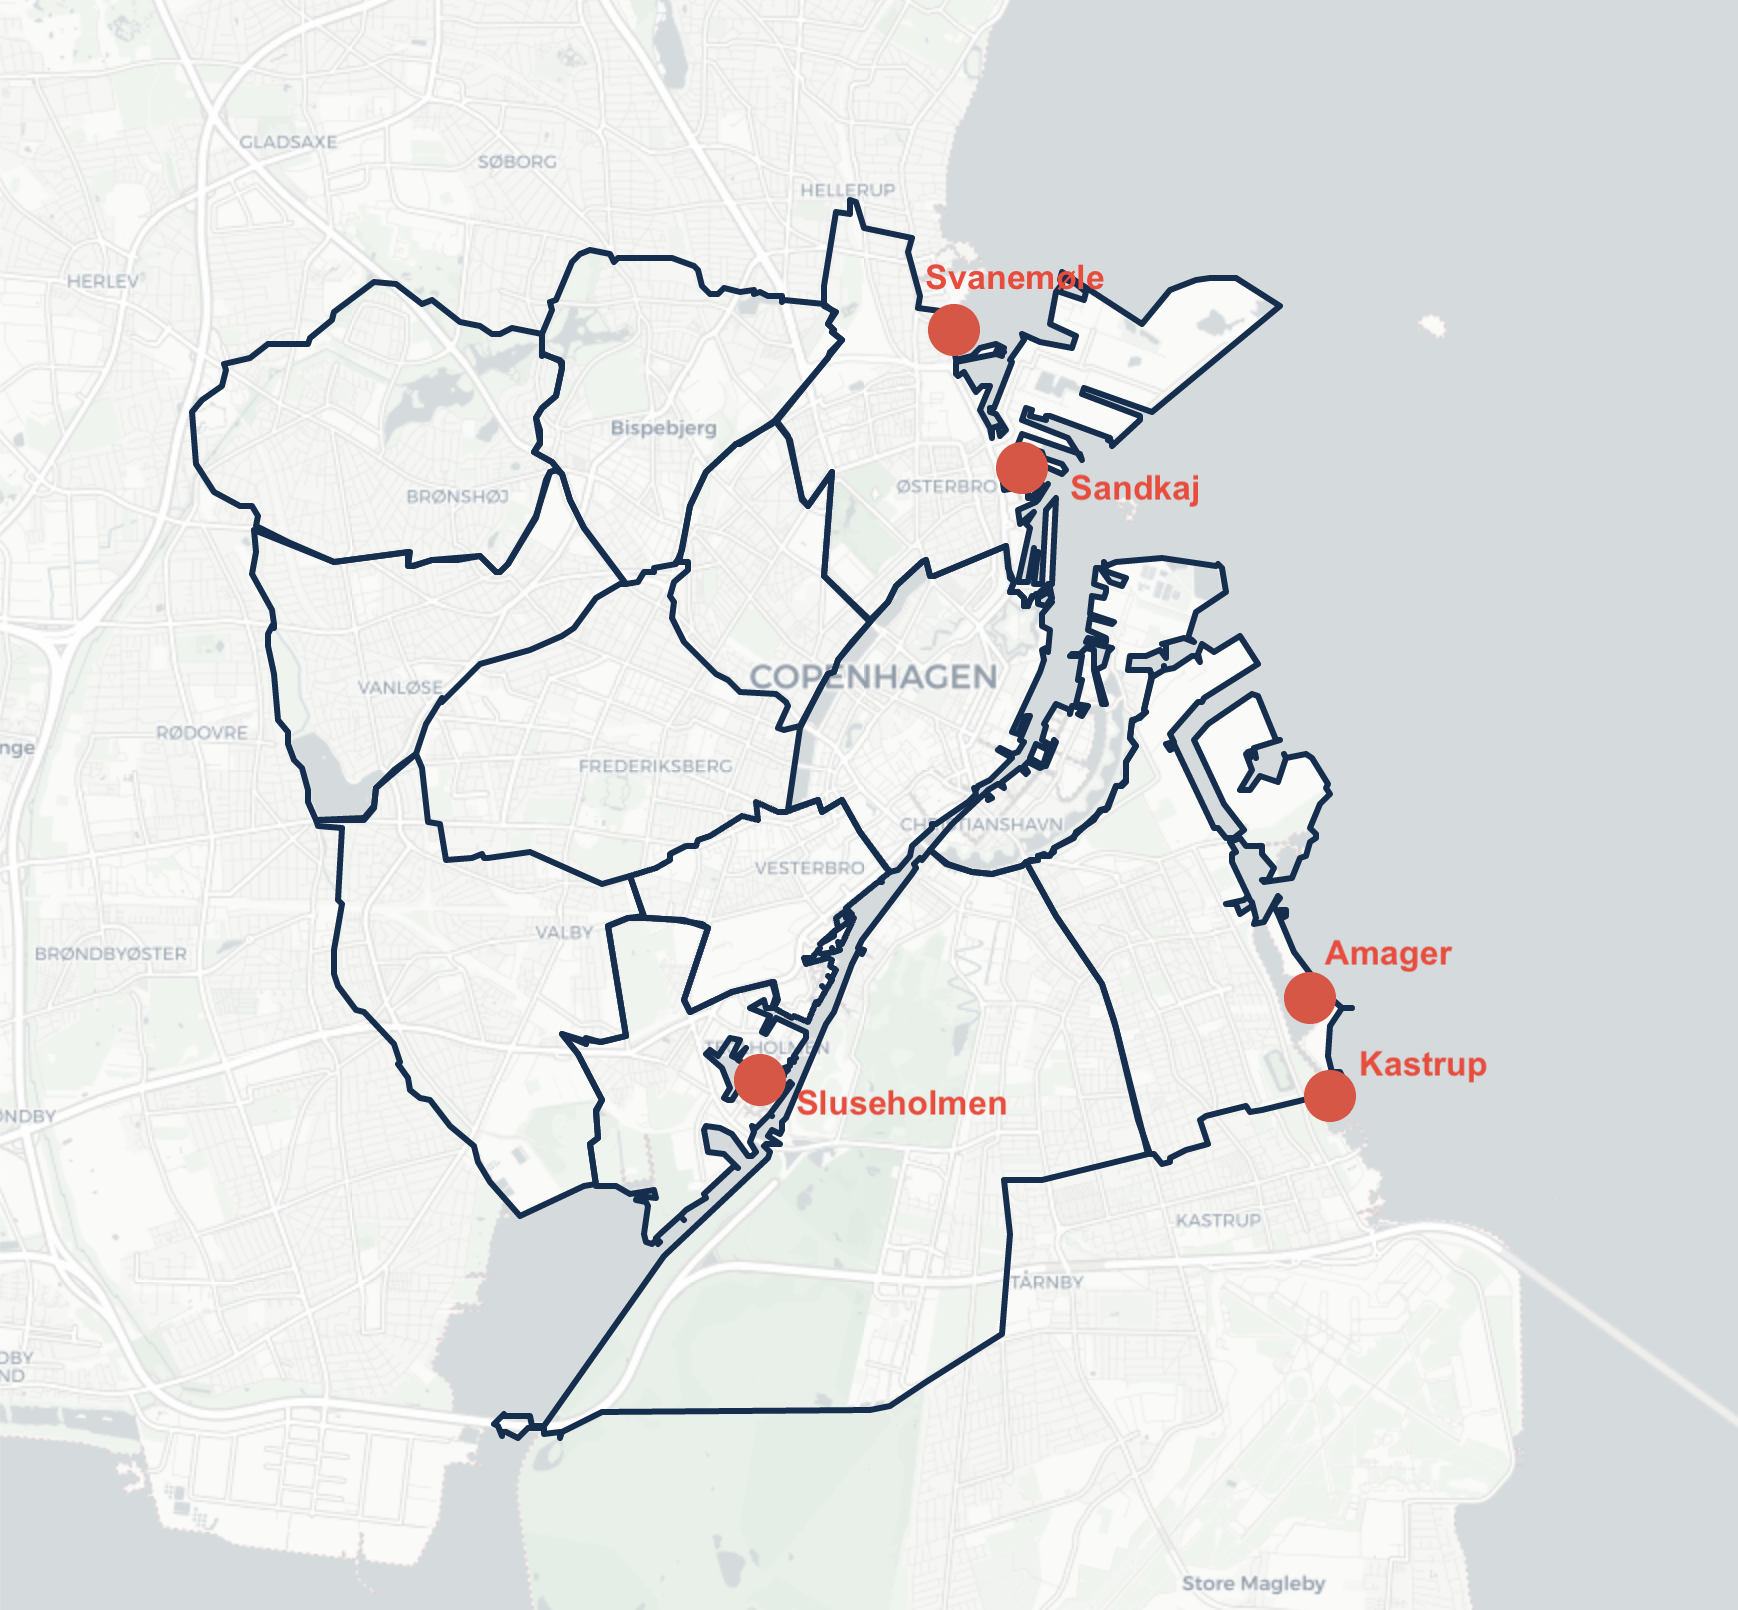
\includegraphics[width=0.8\textwidth]{copenhagen_bs_shortlist.png}
	\caption{\textit{A map of Copenhagen with the shortlisted blue spaces (in red) in their respective}}
	  \label{fig:ubs}
\end{figure}

\bisection{Sandkaj Harbour Bath} is open for swimming year-round. It is located in the Nordhavn neighbourhood of the Østerbro district, which is referred to as ``the newer part of town’’, a new and exciting area where cafes and restaurants keep opening and create a buzzing feel around the bathing zone” \parencite{visitcopenhagen_baths}.

\bisection{Svanemøle Strand} is also located in the Østerbro district north of the Sandkaj harbour, the Svanemøle beach opened in 2010. It has sand, a pier, and a promenade. Swimming can take place year-round.

\bisection{Sluseholmen Harbour Bath} is the latest harbour bath to open in 2012. It is a “protective lagoon”\parencite{visitcopenhagen_baths} with four different pools for children, youth, exercising and diving. It is supposedly used mainly by families living in the quiet and new neighbourhood \parencite{bak_2015}, due to it being out of reach compared to popular baths in the centre. This site is interesting because so far, it is intended for the local community and is not (yet?) attracting a wider crowd. Plus, both the neighbourhood and baths are new. This makes it a good location to understand how people are shaping the area, as it develops.

\bisection{Amager Beach} is a sandy beach and also has grassy lawns. It is allowed to barbecue, there are sports facilities, and many waterfront activities like volleyball, kite-surfing and snorkeling. There is a bathhouse open year-round with a wooden deck on one end of the beach.

\bisection{Kastrup Sea Bath} is just south of Amager beach, with views of Saltholm Island and Sweden, equipped with an award-winning architectural structure. It is equipped with changing rooms, showers, lockers, swimming facilities, and people can dive from the structure. The water around the structure is deep and thus not ideal for children or those uncomfortable in deep water.

%%%%%%%%%%%%%%%%%%%%
\subsection{Data collection}
%%%%%%%%%%%%%%%%%%%%

\begin{comment}
The research has the following objectives:
\begin{enumerate}
	\item To understand people's motivations for visiting, or not visiting, a particular UBS
	\item To compare a set of UBS in the city, in terms of the motivations discovered above
	\item To discuss how this knowledge can be used by city planners, to provide UBS that can be used by everyone
\end{enumerate}
\end{comment}

The data collection methods will be a combination of interviews with UBS users and observations of the UBS. See Appendix A for the detailed interview and observation protocols.

\subsubsection{Interviews}

Interviews with UBS users consist of structured, open-ended questions, and are estimated to take a maximum of 30 minutes to complete. The aim of these interviews is to ask users specific questions about the way they use the UBS, their reasons for visiting a particular UBS, their preferences for physical environment (eg. attractiveness of nature, built environment, services) and  social setting (eg. perceptions of other users and activities, feelings of safety or belonging), their perception the UBS in these terms, and what barriers may inhibit them from using UBS.

Limiting the interviews to 30 minutes will allow me to collect a maximum of responses compared to more lengthy ones. And compared to surveys, a qualitative interview approach will enable me to explore in depth the motivations behind people's perceptions of the space.

I aim to collect a minimum of 15 interviews per UBS, so a total of 45 across the 3 sites.

\subsubsection{Observations}

Interviews will be combined with direct observations of human activity, signs of human activity, and qualities of the site. Previous research have identified observable factors that inhibit use of urban green space, like infrastructure attracting specific user groups (eg. sports equipment), trash like broken glass (REF), vandalism (REF), or the appearance of the surrounding nature (REF).

Observations of human activity will collect information on the type of activities people are carrying out, such as swimming, playing sports, walking, sitting, socialising, and so on. I will pay particular attention to conflicting uses and user groups, antisocial or illicit behaviour, the sociability of people (whether they are on their own, in pairs or groups), noise levels of users, and demographics (age, sex).

The signs of human activity are similar, but the activities are not happening during the observation either because they happen more slowly over time, or at a different time of day or week. For example, advertised events or community groups, broken glass, or XXX.

% but this is more like an evaluation of the human/social activity. maybe i mean physical preferences?
The qualities of the UBS are anything that impact the appearance of the UBS, and that could be interpreted as particularly attractive or repulsive to certain people.
For example, the built environment (infrastructure like paths, equipment like benches and trash cans, services like toilets), the quality of the water, the surrounding environment (nature, roads, shops, restaurants), or the noise levels coming from certain groups or the surroundings.

Altogether, these observations say something about the character of the UBS and how different groups of people socially interpret it. This feeds directly into people's judgement of whether to use the space.

%%%%%%%%%%%%%%%%%%%%
\subsection{Data analysis}
%%%%%%%%%%%%%%%%%%%%

Quantitative data from the observations and closed-answer responses will be entered into a spread sheet for statistical analysis. Pivot tables are a popular way to organise data to make it easier to find patterns.
% Statistical analysis ??
% Spatial analysis ??

Qualitative field observations and open-ended survey responses will be encoded. The coding scheme will be updated after each day of data collection, and serve to identify key concepts. When the encoding is complete, clustering may be applied to the codes, as recommended by Miles and Huberman \parencite{miles1994qualitative}.

After the data has been organised, encoded and analysed, I will do a comparative analysis across the UBS. A distinction will also be made between the UBS where data was collected, and other UBS  survey respondent have mentioned. 

%The results will be organised spatially to convey how perceived access varies across the city.

The results from the analysis will be highly subjective, since that is the nature of perceptions. Therefore, I will not be producing an exhaustive representation of people's experiences of UBS across Copenhagen, but rather a more holistic discussion based on access and justice.

\pagebreak
\section{Timeline and feasibility}

Many more people spend time at the water in summer compared to than winter. Therefore, I aim to collect my data starting in August and going up to October. This should allow me to capture a wide range of users and uses. Even though swimming culture is big in Denmark and people do use UBS all year, winter swimmers are a very particular group of people compared to the more general population I plan to study.

\begin{figure}[h]
\begin{ganttchart}[
hgrid,
vgrid,
expand chart=\textwidth,
time slot format=isodate-yearmonth,
time slot unit=month
]{2022-03}{2023-06}
\gantttitlecalendar{year, month} \\
\ganttbar{Thesis proposal}{2022-03}{2022-06} \\
\ganttbar{Design observation guide}{2022-07}{2022-07} \\
\ganttbar{Design surveys}{2022-07}{2022-07} \\
\ganttbar{1st visit to UBS}{2022-08-01}{2022-08-31} \\
\ganttbar{Pilot observations \& surveys}{2022-08-01}{2022-08-31} \\
\ganttbar{Data collection}{2022-08}{2022-10} \\
\ganttbar{Literature review}{2022-09}{2022-11} \\
\ganttbar{Data analysis}{2022-12}{2023-03} \\
\ganttbar{Writing report}{2023-03}{2023-06} \\
\ganttmilestone{Thesis defence}{2023-06}
\end{ganttchart}
\caption{Timeline for the research}
\end{figure}


\printbibliography

\appendix

\section{Appendix A: Data Collection Protocols}

\subsection{Observation Protocol}

\hl{TODO}

\subsection{Survey Protocol}

\hl{TODO}

\end{document}

%%%%%%%%%%%%%%%%%%%%%%%%%%%%%%%%%%%%
%				COMMENTS
%%%%%%%%%%%%%%%%%%%%%%%%%%%%%%%%%%%%

\begin{comment}
THESIS NOTES

Limitations:
- Observations done by a single person may not be reliable, would be more reliable and richer if conducted by 2 researchers who could debrief their observations and discuss their interpretations
- Only interviewed users, and not non-users of UBS
\end{comment}
